\documentclass[12pt]{kjleehw}

\usepackage{subfigure}
\usepackage{CJKutf8}
\usepackage{listings}
\usepackage{verbatim}
\usepackage{enumerate}
\usepackage{amsmath, amsfonts, amssymb, mathtools}  % AMS數學模組
\usepackage{bm}
\usepackage{pagecolor}
\usepackage{changepage}
\usepackage{listings}
% \lstset{
%   backgroundcolor=\color{gray},
% }
\definecolor{codegreen}{rgb}{0,0.6,0}
\definecolor{codegray}{rgb}{0.5,0.5,0.5}
\definecolor{codepurple}{rgb}{0.58,0,0.82}
\definecolor{backcolour}{rgb}{0.95,0.95,0.92}
\lstdefinestyle{mystyle}{
    backgroundcolor=\color{backcolour},   
    commentstyle=\color{codegreen},
    keywordstyle=\color{magenta},
    numberstyle=\tiny\color{codegray},
    stringstyle=\color{codepurple},
    basicstyle=\footnotesize,
    breakatwhitespace=false,         
    breaklines=true,                 
    captionpos=b,                    
    keepspaces=true,                 
    numbers=left,                    
    numbersep=5pt,                  
    showspaces=false,                
    showstringspaces=false,
    showtabs=false,                  
    tabsize=2
}
 
\lstset{style=mystyle}

\renewcommand{\figurename}{Figure}
\renewcommand{\tablename}{Table}

\renewcommand\appendix{\par
\setcounter{section}{0}
\setcounter{subsection}{0}\today\today
\setcounter{figure}{0}
\setcounter{table}{0}
\renewcommand\thesection{Appendix \Alph{section}}
\renewcommand\thefigure{\Alph{section}\arabic{figure}}
\renewcommand\thetable{\Alph{section}\arabic{table}}
}

% -- bibtex 不要出現 Reference 的 title,我用 Section 來作
\usepackage{etoolbox}
\patchcmd{\thebibliography}{\section*{\refname}}{}{}{}
% --

\setlength{\abovecaptionskip}{10pt}
\setlength{\belowcaptionskip}{10pt}

% 首段空格
\setlength{\parindent}{0em}

% English Font and color, rm/ss/tt
\renewcommand{\familydefault}{\rmdefault} 
% \definecolor{EyeBlack}{HTML}{222222}
% \definecolor{EyeGreen}{HTML}{76D38F}
% \pagecolor{EyeBlack}
% \color{EyeGreen}

% ----
% ----

\begin{document}

%  bsmi (明體), bkai (楷書), DFKai-SB
\begin{CJK}{UTF8}{bkai} 
\title{\textbf{Optimization in Engineering \\ Appendix - Run ANSYS Workbench in batch mode}}
% \lhead{Optimal Design}
% \rhead{System Optimization Lab.}

% \tableofcontents

% -----------------------------------------------
\section{Introduction}

This document is only used for academic purpose and released in MIT License. We demonstrate how to change the ANSYS Workbench project's parameters (or variables) and execute the simulation in batch mode (command line) with Python script under Windows OS.\\

We are \underline{\textbf{not}} encourage students to use commercial softwares. But the basic concept of the integration of your program with other softwares should be similiar.

% -----------------------------------------------
\section{Install ANSYS Student}

Download the ANSYS Student Software from : \textbf{https://www.ansys.com/academic/free-student-products} and follow the installation instruction in the website.

\begin{figure}[h]
	\centering
	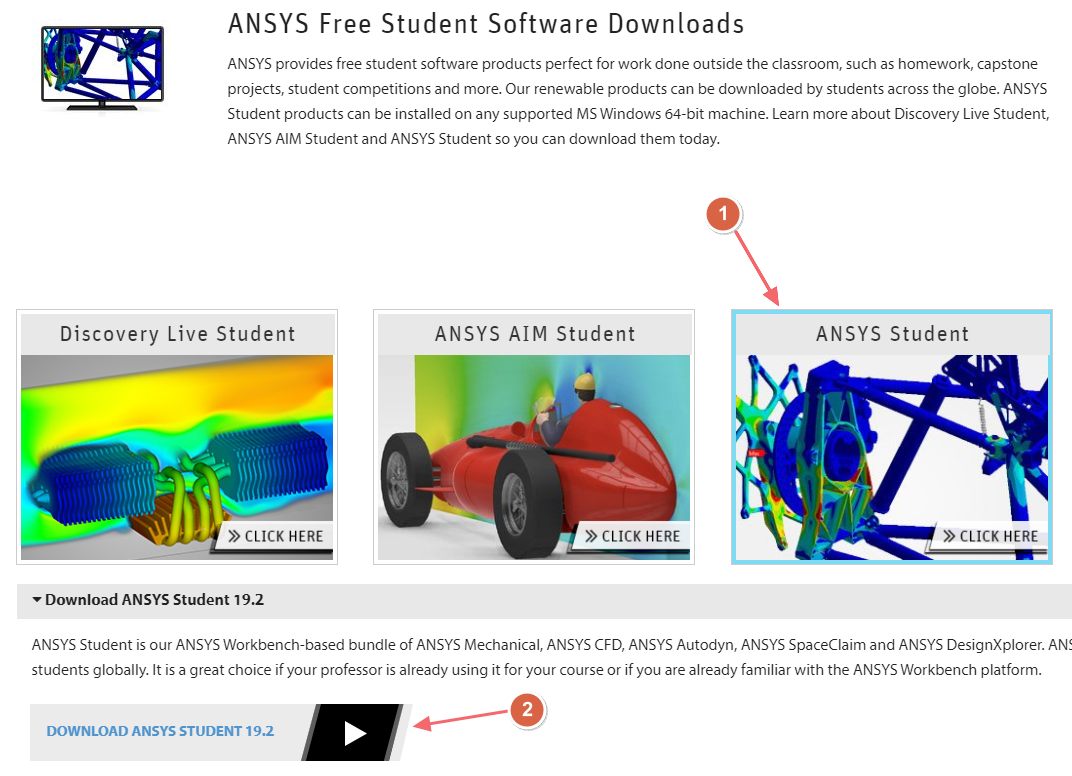
\includegraphics[scale=0.4]{figure/download_ansys.png}
	\caption{ANSYS Free Student Software Downloads}
	\label{fig:download_ansys}
\end{figure}

The ANSYS Student Software is provided a twelve-month renewable license and limited with 32k nodes/elements in Structure Analysis, 512k nodes/cells in Fluid Analysis.

% -----------------------------------------------
\section{Example}

\subsection{Download}

Download the example file from CEIBA or GitHub :
\textbf{https://github.com/solab-ntu/batch-ansys-workbench} .The file \textbf{example.zip} should contain at least 4 items which include following files/folder:

\begin{itemize}
  \item model\_v192\_student.wbpj
  \item model\_v192\_student\_files/
  \item batch\_run\_ansys.py
  \item batch\_cmd.bat
\end{itemize}

The project file (model\_v192\_student.wbpj) should only be opened in ANSYS Student v19.2 or newer version.

\subsection{Problem Description}

In this project file, we construct a cantilever beam which has three sections as shown in Figure \ref{fig:cantilever}. Each section has a circle sketch and uses the diameter size as the design variables.\\

\begin{figure}[h]
	\centering
	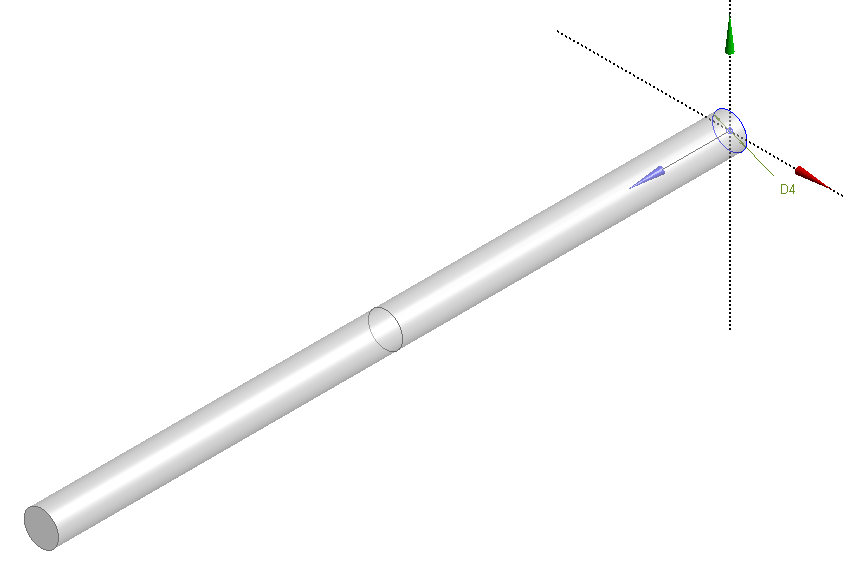
\includegraphics[scale=0.4]{figure/cantilever.png}
	\caption{Geometry}
	\label{fig:cantilever}
\end{figure}

In simulation, we fixed one end of the beam and apply a 100 [N] force (+x) on the other end. The stress and deformation distribution are shown in Figure \ref{fig:anslysis}. Then we can retrieve the response values to Parameter Set Table, as shown in Figure \ref{fig:parameters}.

\begin{figure}[h]
	\centering
  \subfigure[Stress Distribution]{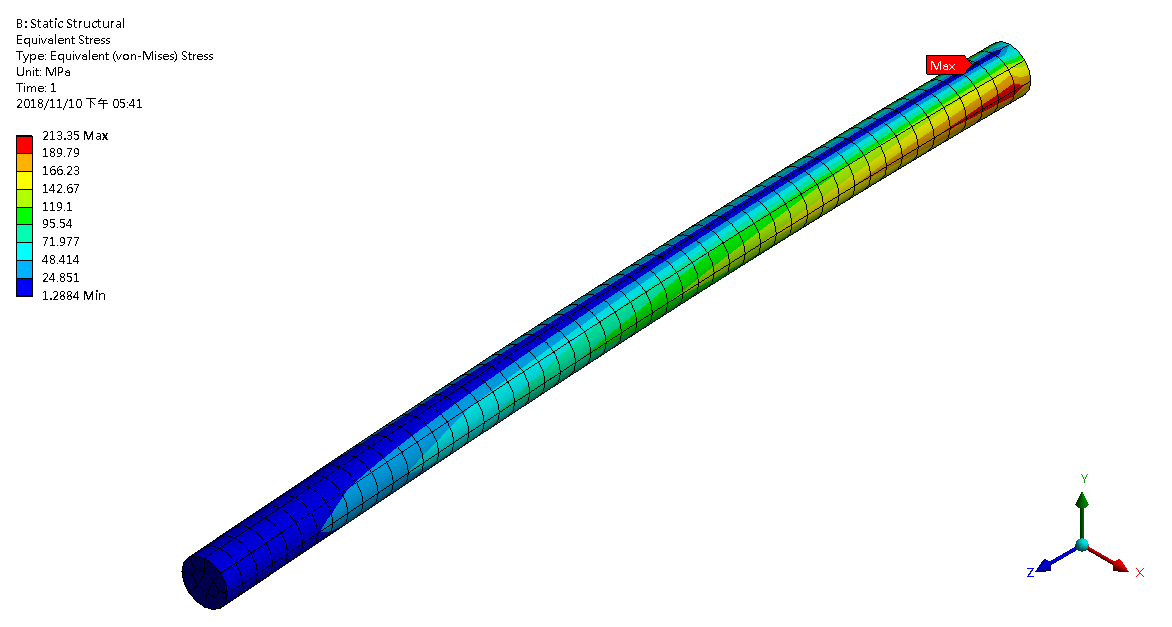
\includegraphics[height=4.2cm]{./figure/stress.png}}
  \subfigure[Max. Displacement]{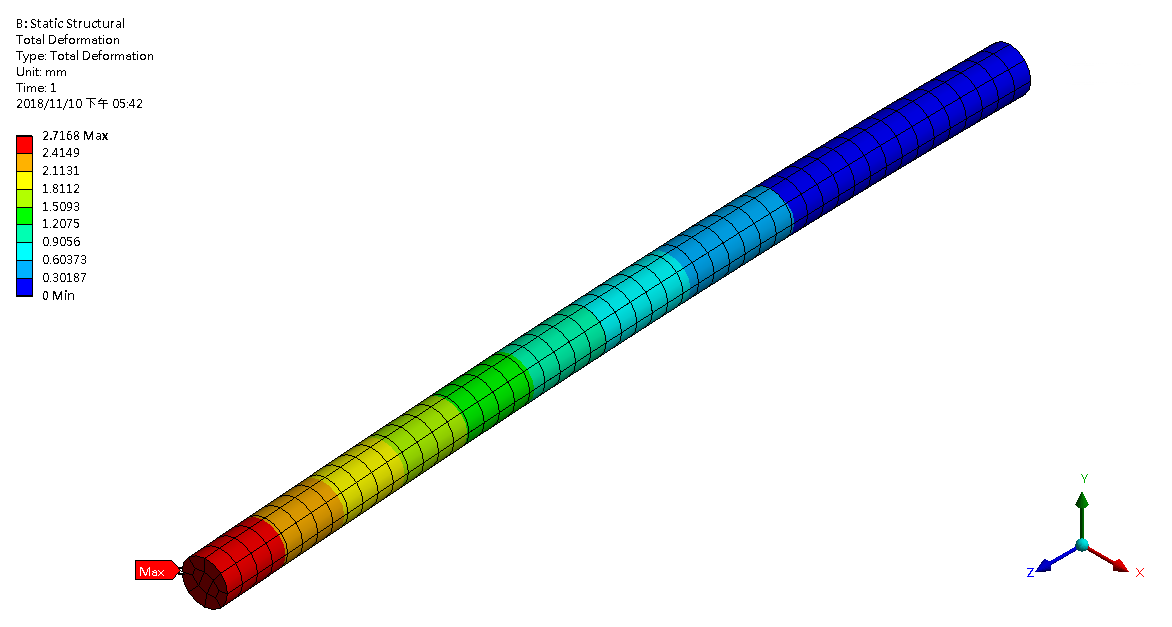
\includegraphics[height=4.2cm]{./figure/disp.png}}
  \caption{Analysis Result}
  \label{fig:anslysis}
\end{figure}

\begin{figure}[h]
	\centering
	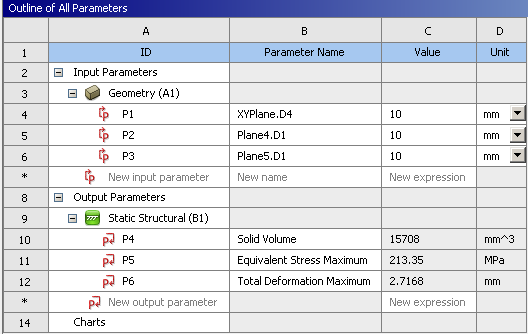
\includegraphics[scale=0.65]{figure/parameters.png}
	\caption{Parameters}
	\label{fig:parameters}
\end{figure}

\subsection{Batch Mode}

\begin{itemize}
  \item batch\_run\_ansys.py

Before start running batch mode. We need to ckeck the project file location in the script. This file path might be different in your computer.

\lstinputlisting[language=Python, firstline=1, lastline=4]{./code/batch_run_ansys.py}

Then we can decide which parameter should be changed and modify the value by the "Expression" argument.

\lstinputlisting[language=Python, firstline=5, lastline=17, firstnumber=5]{./code/batch_run_ansys.py}

After updating the project. We can use Python file I/O function to write out the parameter's information to a plain text file.

\lstinputlisting[language=Python, firstline=22, lastline=30, firstnumber=22]{./code/batch_run_ansys.py}

\end{itemize}

\begin{itemize}
  \item batch\_cmd.bat
  \lstinputlisting[language=Python]{./code/batch_cmd.bat}

  The first part of this .bat file is the path of ANSYS WB program, and the others mean running the program with batch\_run\_ansys.py in batch mode. This two files (batch\_run\_ansys.py and batch\_cmd.bat) should be placed in the same folder.
\end{itemize}

After double clicking batch\_cmd.bat. It will appear two MS-DOS windows as shown in Figure \ref{fig:batch}, and create output.txt when it finished. The output.txt will contain the parameter's information of the project file. \\

For the detailed operation procedure, please check the video : \\
\textbf{https://www.youtube.com/watch?v=jGWYmR0uqtU}

\begin{figure}[h]
	\centering
	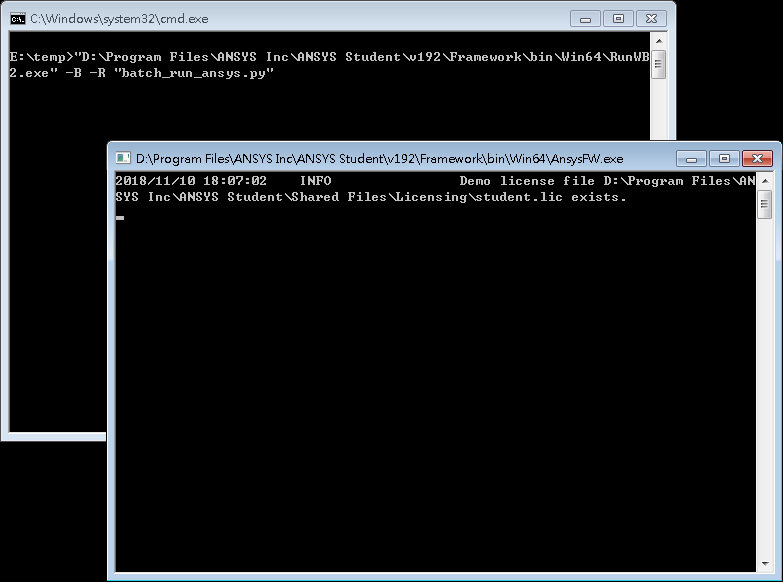
\includegraphics[scale=0.5]{figure/batch.png}
	\caption{Execute batch\_cmd.bat}
	\label{fig:batch}
\end{figure}

\begin{figure}[h]
	\centering
	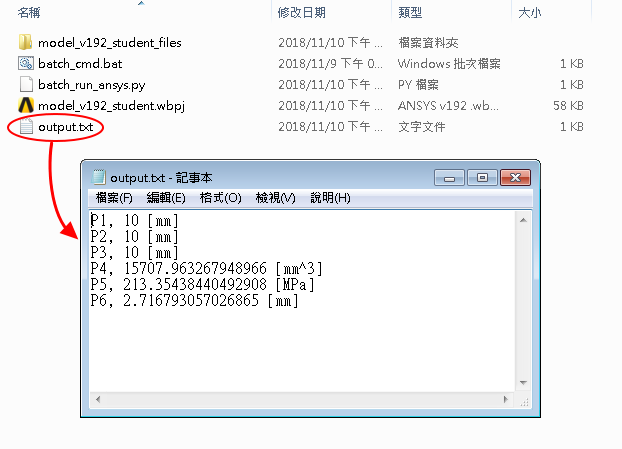
\includegraphics[scale=0.6]{figure/output.png}
	\caption{Output text file}
	\label{fig:output}
\end{figure}

\newpage

% -----------------------------------------------
\clearpage
\end{CJK}
\end{document}
